\documentclass{article}

\usepackage[utf8]{inputenc}
\usepackage[T1]{fontenc}

\usepackage{lmodern}
\usepackage{textcomp}
\usepackage{courier}

\usepackage{amsmath}
\usepackage{stmaryrd}
\usepackage{tikz}
\usetikzlibrary{positioning,%
  shapes.geometric,%
  shapes.misc,%
  calc,%
  fit,%
  decorations,%
  decorations.pathreplacing,%
  backgrounds,%
  arrows,%
  automata,%
  trees
}

% define colors used by presentation theme AND article
\xdefinecolor{bordeaux}{RGB}{128,0,50}
\xdefinecolor{niceblue}{RGB}{13,41,79}
\xdefinecolor{nicegreen}{RGB}{13,79,18}
\xdefinecolor{niceviolet}{RGB}{79,13,74}
\colorlet{maincolor}{orange}
\colorlet{alertedcolor}{red}
\colorlet{examplecolor}{green!50!black}

% color system
% - color!9 used as light fill color (e.g. for block content)
% - color!18 used as default fill color (e.g. for state)
% - color!30 used as highlight fill color (e.g. for block header)
% - color!50 used as strong highlight fill color (e.g. for header row)

\usepackage{tikz}

\usepackage{dtklogos}

\begin{document}
  \newcommand{\icon}[1]{%
    \tikz\draw[very thick, line join=round]
      (-.5,.5) -- ++(.7,0) -- ++(.3,-.3) --
      ++(-.3,0) -- ++(0,.3) -- ++(.3,-.3) -- ++(0,-.8) -- ++(-1,0) -- cycle
      ++ (0,-.3) node[fill, text=white,
        inner sep=2pt, minimum width=8mm, anchor=center] {#1}
      ++ (.1,-.3) -- ++(.8,0) -- ++(0,-.1)
      -- ++(-.8,0) -- ++(0,-.1)
      -- ++(.8,0) -- ++(0,-.1)
      -- ++(-.8,0) -- ++(0,-.1)
      -- ++(.8,0);
  }

  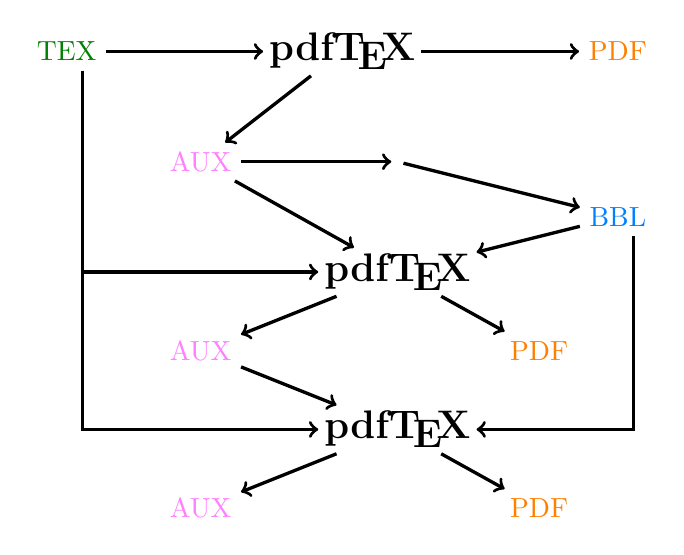
\begin{tikzpicture}[
      on grid,
      node distance=14mm and 35mm,
      engine/.style={
        node font=\rmfamily\Large\bfseries,
        inner sep=2pt
      }
    ]
    \node[examplecolor] (tex) {\icon{TEX}};
    \node[right=of tex, engine]
      (pdfTeX1) {pdf\TeX};
    \node[right=of pdfTeX1, maincolor] (pdf1) {\icon{PDF}};
    \node[below=of pdfTeX1, xshift=-18mm, color=-examplecolor] (aux1) {\icon{AUX}};
    \node[right=25mm of aux1, engine] (BibTeX) {\BibTeX};
    \node[right=28mm of BibTeX, yshift=-7mm, color=-maincolor] (bbl) {\icon{BBL}};
    \node[below=of BibTeX, engine]
      (pdfTeX2) {pdf\TeX};
    \node[below=10mm of pdfTeX2, xshift=-25mm, color=-examplecolor] (aux2) {\icon{AUX}};
    \node[below=10mm of pdfTeX2, xshift=18mm, maincolor] (pdf2) {\icon{PDF}};
    \node[below=10mm of aux2, xshift=25mm, engine] (pdfTeX3) {pdf\TeX};
    \node[below=10mm of pdfTeX3, xshift=-25mm, color=-examplecolor] (aux3) {\icon{AUX}};
    \node[below=10mm of pdfTeX3, xshift=18mm, maincolor] (pdf3) {\icon{PDF}};
    \draw[very thick]
      (tex) edge[->] (pdfTeX1);
    \draw[very thick]
      (pdfTeX1) edge[->] (aux1);
    \draw[very thick]
      (pdfTeX1) edge[->] (pdf1);
    \draw[very thick]
      (aux1) edge[->] (BibTeX)
      (BibTeX) edge[->] (bbl);
    \draw[very thick]
      (aux1) edge[->] (pdfTeX2)
      (bbl) edge[->] (pdfTeX2);
    \draw[->, very thick] (tex.south) ++ (.2,0) |- (pdfTeX2);
    \draw[very thick]
      (pdfTeX2) edge[->] (pdf2)
                edge[->] (aux2);
    \draw[very thick]
      (aux2) edge[->] (pdfTeX3);
    \draw[very thick, ->]
      (tex.south) ++ (.2,0) |- (pdfTeX3);
    \draw[very thick, ->]
      (bbl.south) ++ (.2,0) |- (pdfTeX3);
    \draw[very thick]
      (pdfTeX3) edge[->] (aux3)
                edge[->] (pdf3);
  \end{tikzpicture}
\end{document}